\section{Casos de Uso}


\begin{enumerate}
	\item {Escoger opción del menú juego}
	\item {Escoger opción reglas}	
	\item{Escoger opción desarrolladores}
	\item{Escoger opción puntaje}
\end{enumerate}

\section{Caso}Escoger  opción del menú juego.\newline\newline
Descripcion: En este caso de uso se escogerá las opciones para inicializar el juego y se verán  las diferentes  puntuaciones y las reglas del mismo.

	\subsection{Escenario}
	 Escoger la opción incorrecta que no va corresponder con los requerimientos del usuario.\newline \newline
Actor: jugador.\newline
Acciones: Ingresar a la opción juego.\newline
Resultado: no permite inicializar el juego.\newline

\subsection{Escenario}
Escoger la opción correcta que permita iniciar el  juego, ingreso exitoso.\newline\newline
Actor: jugador.\newline
Asunciones:  Se asume  que la opción escogido fue la correcta.\newline
Resultado: Se iniciara la ventana con las opciones del juego exitosamente.
 
\subsection{Escenario}
 
Escoger el nivel..\newline\newline
Actor: jugador
Asunciones: Vamos asumir que se escogió el nivel correctamente.\newline
Acciones: El actor dará clic en el botono siguiente.\newline
Resultado: Presentara la nueva ventana con el juego cargado.\newline

\subsection{Escenario}
Jugar buscaminas\newline \newline
Actor: jugador\newline
Asunciones: Vamos asumir que el actor ha ingresado correctamente al juego.\newline
Acciones: Presiona una casilla aleatoriamente.\newline
Resultado: el cronometro empieza a correr entonces empieza el juego.\newline

\subsection{Escenario}
Reiniciar.\newline \newline
Actor: Jugador. \newline
Asunciones: Se asume que se dio clic en el botón correcto.\newline
Acciones: El  juego vuelve a cargarse a partir de cero.\newline
Resultado: Presenta una tablero nuevo con todos las minas ocultas.\newline

\subsection{Escenario}
Salir.\newline \newline
Actor: jugador.\newline
Asunciones: Se asume que se dio clic en el botón  correcto.\newline
Acciones: Destruye toda las actividades del juego.\newline
Resultado: Salir exitosamente  de la consola del juego.\newline
\newpage


\section{Caso} Escoger opción reglas\newline\newline
Descripción: en esta opción se muestran todas las reglas del juego

\subsection{Escenario}
Se presionara la opción regla que es del juego.\newline \newline
Actor: Jugador.\newline
Asunciones: Se asume que ha entrado a la opción regla con éxito.\newline
Acciones: Se muestran todas las reglas del juego.\newline
Resultado: El jugador puede leer las reglas del juego.\newline

\section{Caso}
Escoger opción puntaje.\newline \newline
Descripción: Se conoce quienes tienes el tiempo en todos los juegos creados.
\subsection{Escenario}
Se presiona la opción puntaje.\newline \newline
Actor: Jugador.\newline
Asunciones: Se asume que el usuario entro a la opción con éxito.\newline
Resultado: Se muestran los nombres con los mejores puntajes.\newline
\begin{figure}[htbp]
\begin{center}
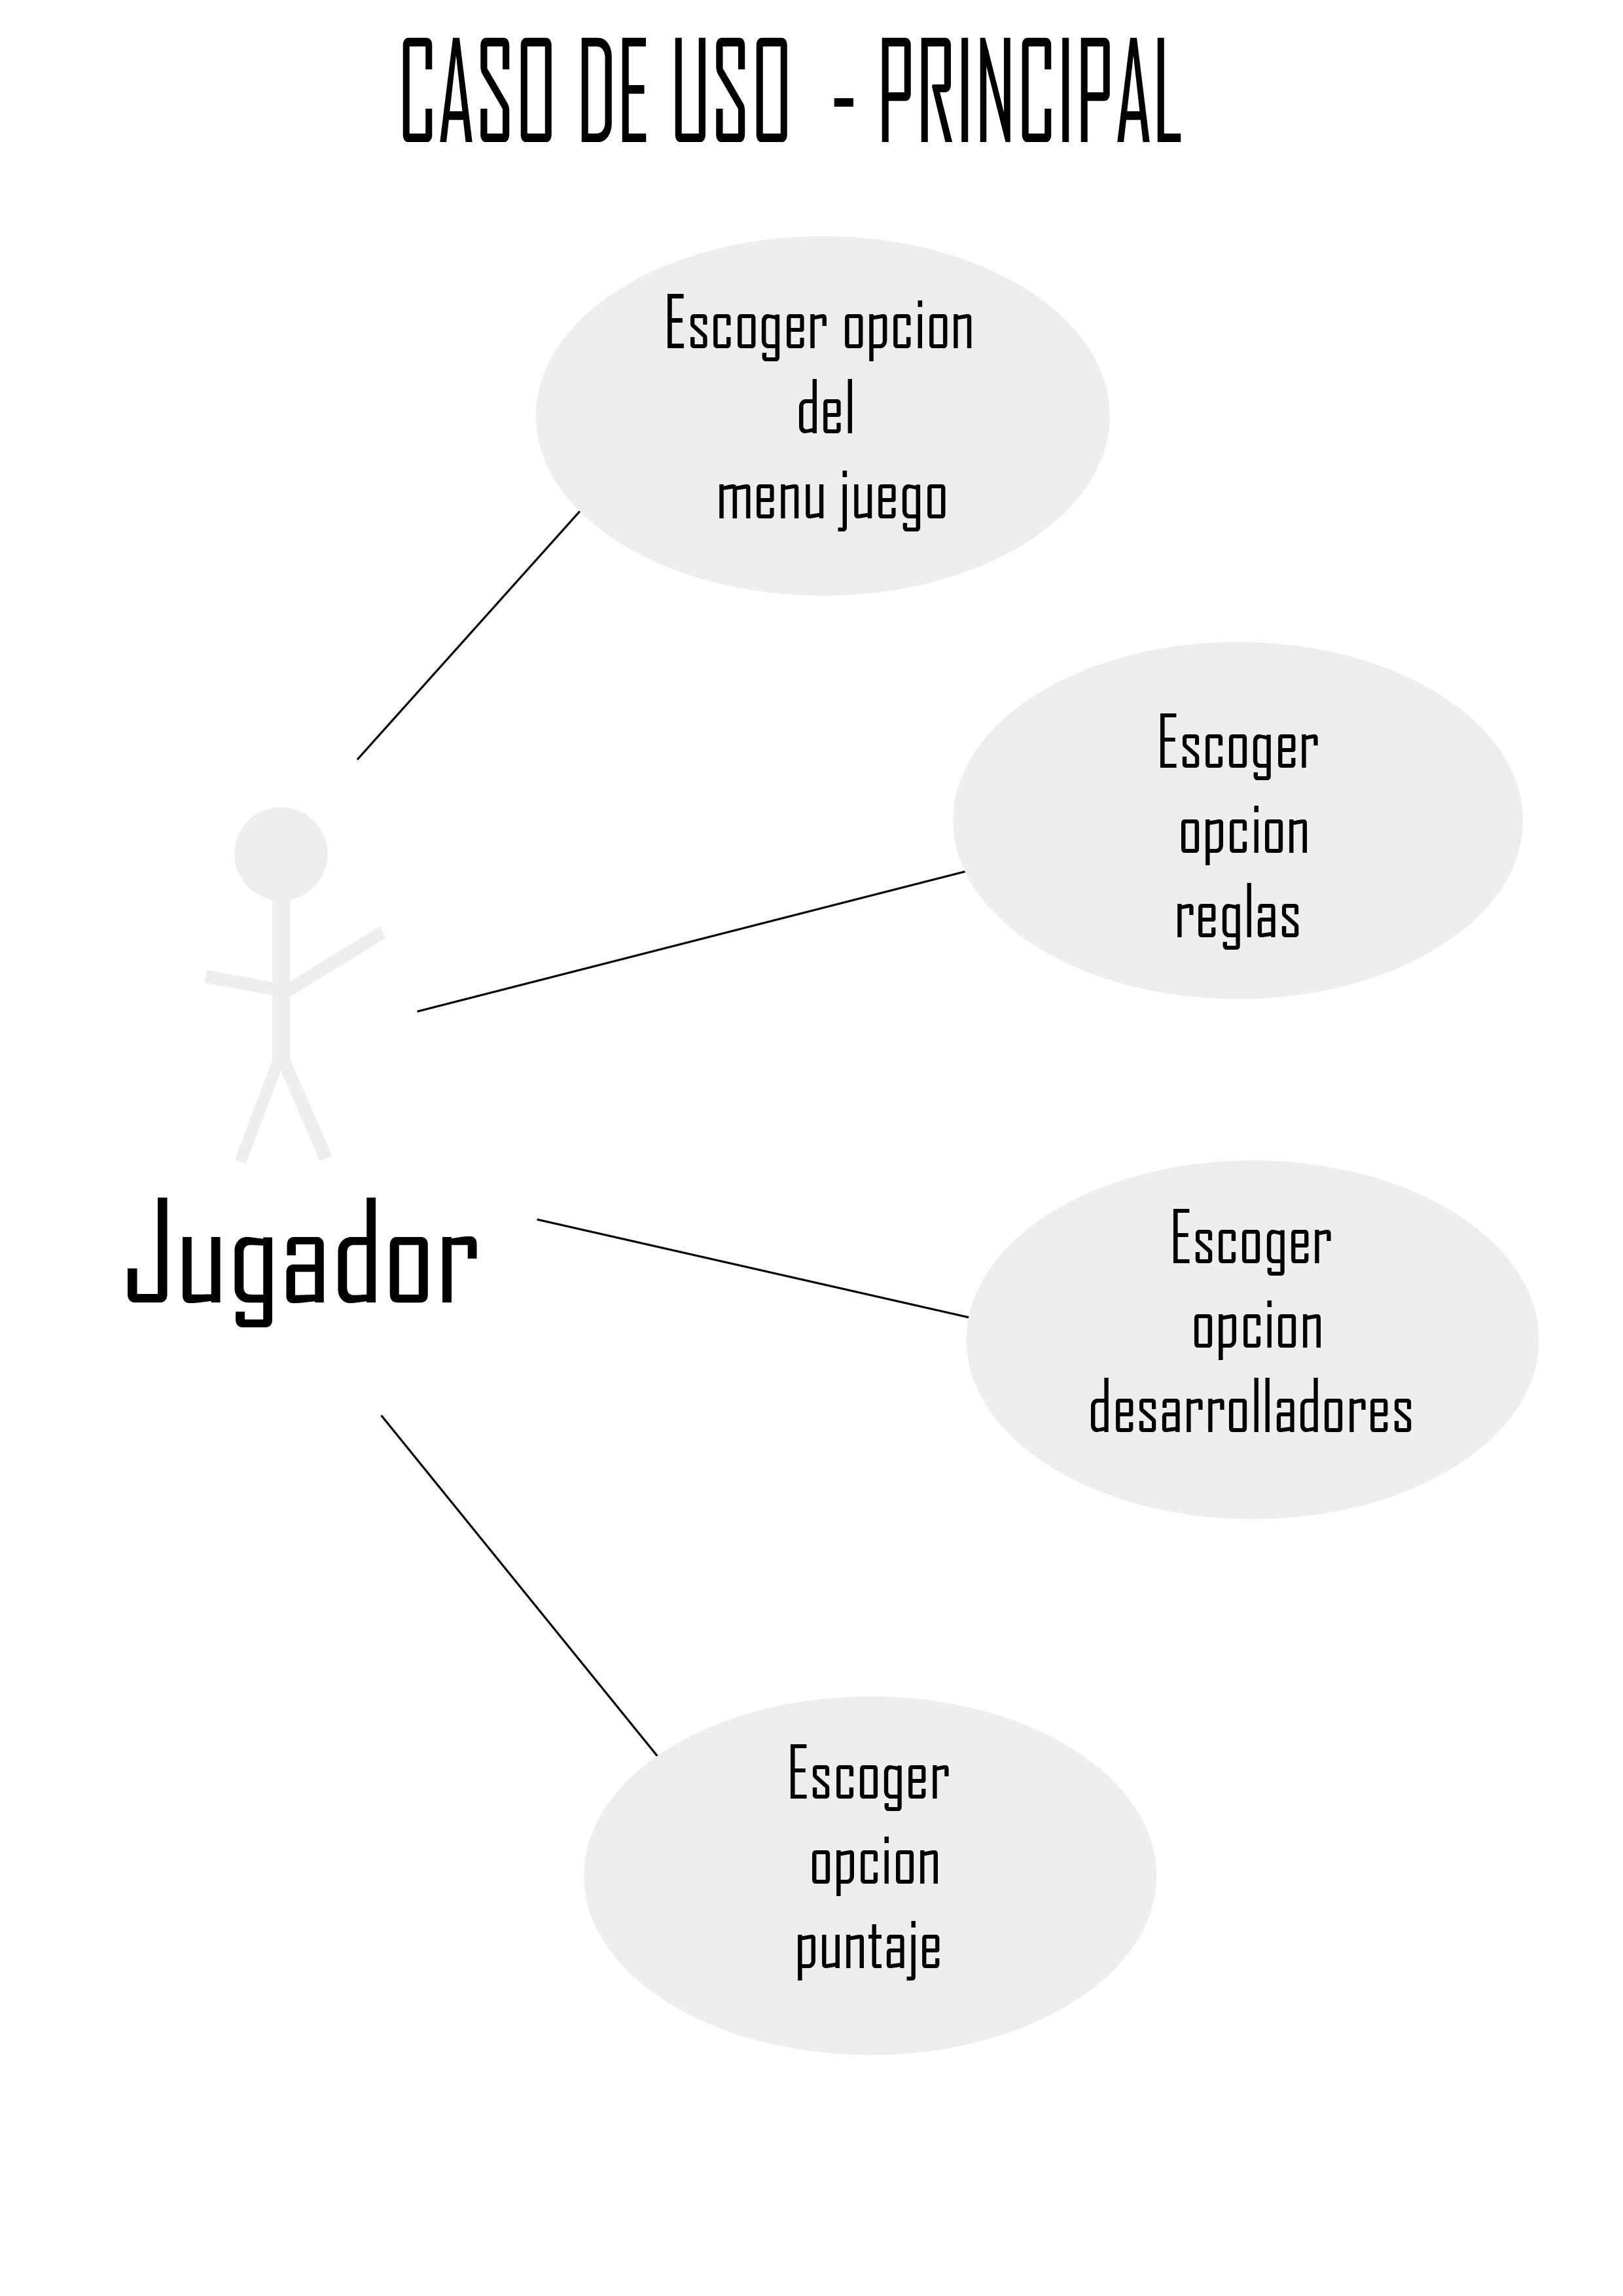
\includegraphics[width=.60\textwidth]{./imagenes/DCU.jpg}
\caption{Diagramas de Casos de usos}
\end{center}
\end{figure}
